\section{Question and contribution}
Company memory should help an assistant decide what to do next, while preserving why the action is justified. The relevant engineering question is whether task-aligned context improves those decisions under an evidence budget. A larger generic company record may contain every necessary fact yet fail to present a usable chain of support to the reader.

We evaluate three visible treatments: \textbf{no company context}, \textbf{general company context}, and \textbf{GTM context}. The domain is marketing decision support. Each treatment feeds the same task, action catalog and output schema to a fixed reader, separately for GPT-6.1 Sol and Claude Opus 5.5. ``Better'' means recovering more of an explicitly defined, feasible and fully evidenced policy-priority objective. It does not mean increased revenue or expert-preferred strategy.

The contribution is an inspectable experiment and benchmark: multi-account decisions, linked prerequisites, approved policy, conflicting observations and a shared resource allowance. We measure the best decision supported by the selected context before measuring the model's returned decision. This distinguishes an information-selection bottleneck from a reader failing to use available evidence. Strong controls include a generic query-word selector, structured Markdown, native GBrain search and full current context. The query-word control is deliberately capable of falsifying the claim that a dedicated GTM architecture is necessary.

\begin{figure}[!ht]
\centering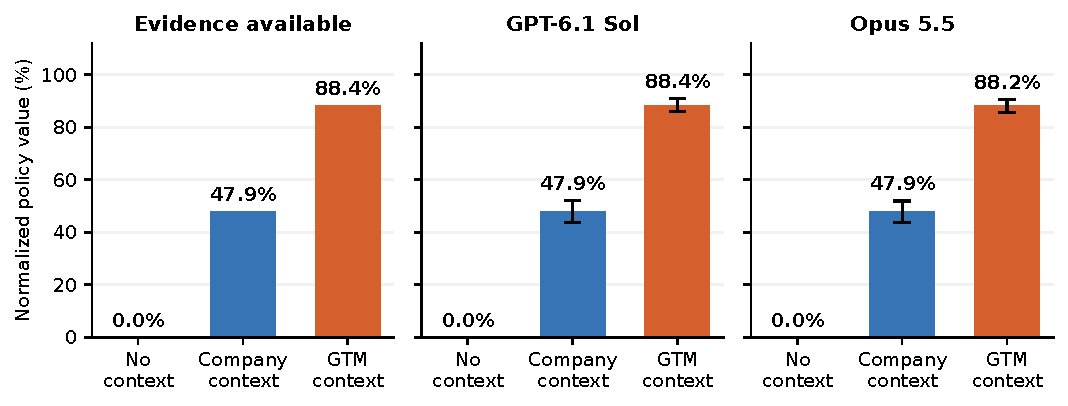
\includegraphics[width=\linewidth]{figures/challenge/headline.pdf}
\caption{The three primary context treatments. Left: the maximum policy value supported by retrieved evidence. Center/right: the grounded feasible value actually returned by each reader. Values are percentages of each positive case's full-information optimum, averaged equally by company. Reader error bars are company-clustered 95\% bootstrap intervals. No-context abstention does not earn positive decision value; negative-case safety is reported separately. Generic query-word closure produces the same GTM inputs and is an explicit control, not additional independent observations.}
\label{fig:headline}
\end{figure}
